\documentclass[border=2pt,tikz]{standalone}
\usepackage[T1]{fontenc}
% Nature Portfolio / Scientific Data shared TikZ style for IRexp figures.
% Width: 183 mm double-column. Typography: Helvetica-class (phv).
\RequirePackage{tikz}
\RequirePackage{pgfplots}
\RequirePackage{xcolor}
\RequirePackage{helvet}
\IfFileExists{sansmathfonts.sty}{\RequirePackage{sansmathfonts}}{}
\renewcommand{\familydefault}{\sfdefault}
\pgfplotsset{compat=1.18}
\usetikzlibrary{
  arrows.meta,calc,positioning,fit,shapes.geometric,shapes.misc,
  backgrounds,shadows.blur,patterns,decorations.pathreplacing
}

% ---- Paul Tol / NMRexp-matched palette ----
\definecolor{nmrBlue}{HTML}{4A7EBB}
\definecolor{nmrBlueDark}{HTML}{2E5F8F}
\definecolor{nmrBlueLight}{HTML}{A8C8E8}
\definecolor{nmrPeach}{HTML}{E8B48C}
\definecolor{nmrNavy}{HTML}{1B3D5C}
\definecolor{nmrRed}{HTML}{C44E52}
\definecolor{nmrGreen}{HTML}{3D8B5E}
\definecolor{nmrOrange}{HTML}{D97B32}
\definecolor{ink}{HTML}{1A1A1A}
\definecolor{muted}{HTML}{7A7F85}
\definecolor{note}{HTML}{5C636A}
\definecolor{faint}{HTML}{E8EAEC}
\definecolor{ghost}{HTML}{C5C9CD}
\definecolor{tintBlue}{HTML}{EEF3F8}
\definecolor{tintGreen}{HTML}{EAF4EE}

\newcommand{\NatureFont}{\fontfamily{phv}\selectfont}
\newcommand{\PanelLabel}[1]{%
  {\NatureFont\bfseries\fontsize{8}{9.6}\selectfont #1}%
}
\newcommand{\FigBody}{\NatureFont\fontsize{7}{8.4}\selectfont}
\newcommand{\FigSmall}{\NatureFont\fontsize{5.5}{6.6}\selectfont}
\newcommand{\FigAxis}{\NatureFont\fontsize{7}{8.4}\selectfont}

\tikzset{
  nature arrow/.style={
    -{Latex[length=1.6mm,width=1.3mm]},
    line width=0.55pt, ink
  },
  nature arrow grey/.style={
    -{Latex[length=1.6mm,width=1.3mm]},
    line width=0.5pt, note
  },
  stage card/.style={
    draw=nmrBlueDark, line width=0.7pt, rounded corners=2.2pt,
    fill=white, inner sep=3pt, align=center, font=\FigBody
  },
  stage header/.style={
    fill=nmrBlueDark, text=white, font=\FigBody\bfseries,
    rounded corners=2.2pt, inner sep=2.5pt, align=center
  },
  soft card/.style={
    draw=ghost, line width=0.55pt, rounded corners=2.2pt,
    fill=white, inner sep=3.5pt, align=left, font=\FigBody
  },
}

\pgfplotsset{
  nature axis/.style={
    tick label style={font=\FigSmall, /pgf/number format/assume math mode},
    label style={font=\FigAxis\bfseries},
    title style={font=\FigBody\bfseries, color=ink},
    axis line style={ink, line width=0.5pt},
    tick style={ink, line width=0.45pt},
    major grid style={faint, line width=0.35pt},
    axis x line=bottom,
    axis y line=left,
    enlarge x limits=false,
    clip=false,
  },
  nature hbar/.style={
    nature axis,
    xbar,
    bar width=7pt,
    y=data,
    nodes near coords,
    every node near coord/.append style={
      font=\FigSmall, ink, anchor=west, /pgf/number format/fixed,
      /pgf/number format/1000 sep={,}
    },
    xtick=\empty,
    axis x line=none,
    y axis line style={ink, line width=0.55pt},
    ytick style={draw=none},
    y tick label style={font=\FigBody, ink, anchor=east},
    grid=major x,
    xmin=0,
  },
}

% Auto-generated from frozen_plot_data.json — do not edit by hand.
\newcommand{\IRexpTotal}{121233}
\newcommand{\IRexpStruct}{43060}
\newcommand{\IRexpCommercial}{88545}
\newcommand{\IRexpNMR}{87075}
\newcommand{\IRexpPMC}{119345}
\newcommand{\IRexpChemotion}{1888}
\newcommand{\IRexpNC}{21823}
\newcommand{\IRexpEmpty}{8963}
\newcommand{\IRexpSA}{1897}
\newcommand{\IRexpOther}{5}
\newcommand{\IRexpQuad}{33201}
\newcommand{\NMRexpN}{3370987}
\newcommand{\SDBSN}{54100}
\newcommand{\NISTN}{17000}
\newcommand{\BandMedian}{9}
\newcommand{\TxMAE}{0.0049}
\newcommand{\BandRecallPool}{0.9903}
\newcommand{\ListMatchPool}{0.9848}
\newcommand{\FailRate}{0.0321}

% Band histogram coordinates (x,y)
\newcommand{\BandHistCoords}{
(4,24556)
(6,22989)
(8,18726)
(10,14534)
(12,9959)
(14,7368)
(16,5241)
(18,3899)
(20,3017)
(22,2202)
(24,1822)
(26,1426)
(28,1069)
(30,826)
(32,698)
(34,534)
(36,386)
(38,408)
(40,298)
(42,250)
}

% Element bars
\newcommand{\ElementCommonCoords}{
(43047,8)% C
(38870,7)% O
(36292,6)% N
(12258,5)% S
(5939,4)% F
(7675,3)% Cl
(3923,2)% Br
(959,1)% Si
(859,0)% P
}
\newcommand{\ElementRareCoords}{
(904,8)% I
(270,7)% B
(384,6)% Se
(119,5)% Fe
(73,4)% Te
(64,3)% Sn
(1,2)% Ge
(16,1)% Na
(24,0)% K
}
\newcommand{\ElementCommonLabels}{C,O,N,S,F,Cl,Br,Si,P}
\newcommand{\ElementRareLabels}{I,B,Se,Fe,Te,Sn,Ge,Na,K}
\newcommand{\ElC}{43047}
\newcommand{\ElO}{38870}
\newcommand{\ElN}{36292}
\newcommand{\ElS}{12258}
\newcommand{\ElF}{5939}
\newcommand{\ElCl}{7675}
\newcommand{\ElBr}{3923}
\newcommand{\ElSi}{959}
\newcommand{\ElP}{859}
\newcommand{\ElI}{904}
\newcommand{\ElB}{270}
\newcommand{\ElSe}{384}
\newcommand{\ElFe}{119}
\newcommand{\ElTe}{73}
\newcommand{\ElSn}{64}
\newcommand{\ElGe}{1}
\newcommand{\ElNa}{16}
\newcommand{\ElK}{24}
\newcommand{\TxErrMedian}{0.0}
\newcommand{\TxErrCoords}{
(0.0250,196)
(0.0750,0)
(0.1250,0)
(0.1750,0)
(0.2250,0)
(0.2750,0)
(0.3250,0)
(0.3750,0)
(0.4250,1)
(0.4750,0)
(0.5250,1)
(0.5750,1)
(0.6250,0)
(0.6750,0)
(0.7250,0)
(0.7750,1)
(0.8250,0)
(0.8750,0)
(0.9250,0)
(0.9750,0)
(1.0250,0)
}
\newcommand{\TxErrBinWidth}{0.05000}
\newcommand{\PaperRecallMedian}{1.0}
\newcommand{\PaperRecallCoords}{
(0.0250,3)
(0.0750,0)
(0.1250,0)
(0.1750,0)
(0.2250,0)
(0.2750,0)
(0.3250,0)
(0.3750,0)
(0.4250,1)
(0.4750,0)
(0.5250,0)
(0.5750,0)
(0.6250,0)
(0.6750,0)
(0.7250,0)
(0.7750,0)
(0.8250,0)
(0.8750,1)
(0.9250,0)
(0.9750,0)
(1.0250,115)
}
\newcommand{\PaperRecallBinWidth}{0.05000}
\newcommand{\ListMatchMedian}{1.0}
\newcommand{\ListMatchCoords}{
(0.0250,4)
(0.0750,0)
(0.1250,0)
(0.1750,0)
(0.2250,0)
(0.2750,0)
(0.3250,0)
(0.3750,0)
(0.4250,0)
(0.4750,0)
(0.5250,1)
(0.5750,0)
(0.6250,2)
(0.6750,1)
(0.7250,1)
(0.7750,0)
(0.8250,1)
(0.8750,0)
(0.9250,0)
(0.9750,0)
(1.0250,109)
}
\newcommand{\ListMatchBinWidth}{0.05000}
\newcommand{\FailCtMedian}{0.0}
\newcommand{\FailCtCoords}{
(0.1250,271)
(0.3750,0)
(0.6250,0)
(0.8750,0)
(1.1250,9)
(1.3750,0)
(1.6250,0)
(1.8750,0)
(2.1250,0)
(2.3750,0)
}
\newcommand{\FailCtBinWidth}{0.25000}


\begin{document}
\NatureFont
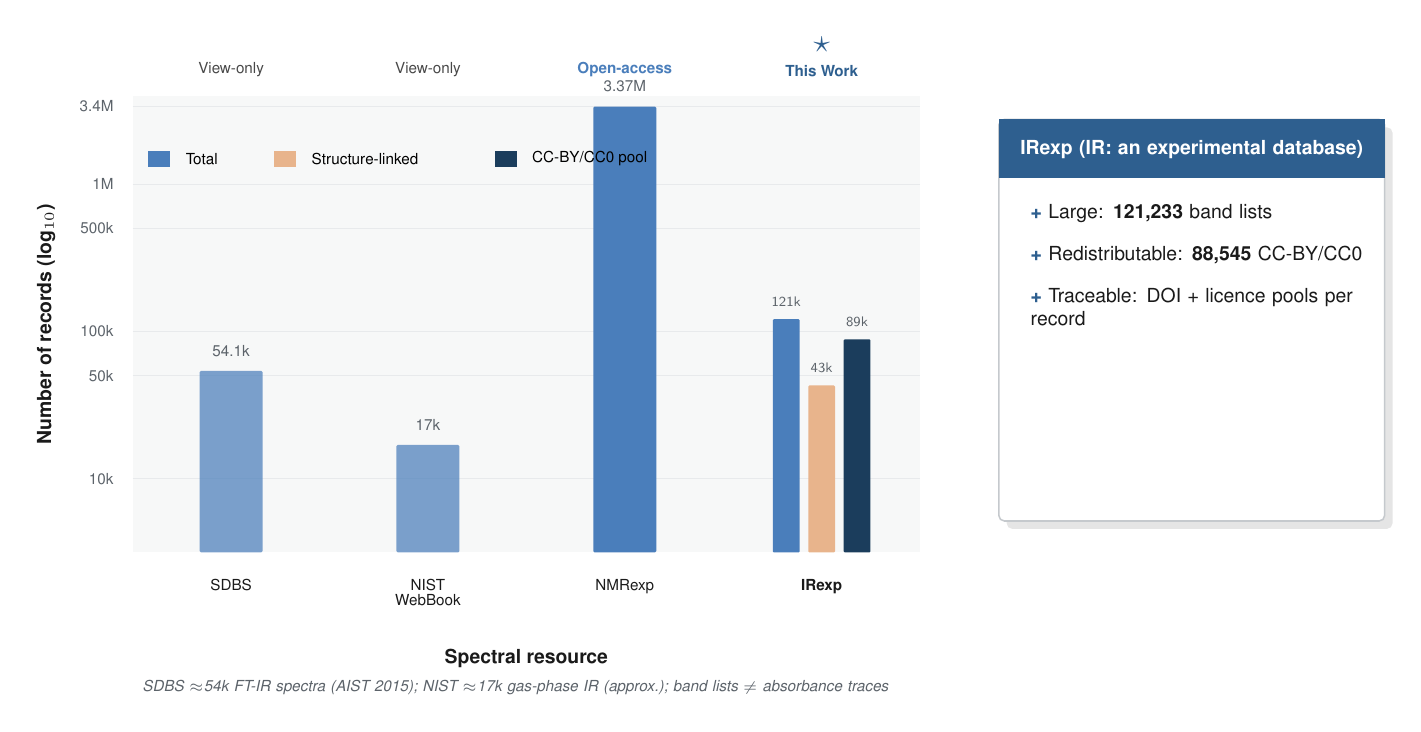
\begin{tikzpicture}[x=1mm,y=1mm]
  \def\W{183}\def\H{92}
  \def\L{18}\def\R{118}\def\B{22}\def\T{80}
  \pgfmathsetmacro{\CW}{\R-\L}
  \pgfmathsetmacro{\CH}{\T-\B}
  \def\logmin{3.5}
  \def\logmax{6.6}
  \pgfmathsetmacro{\logspan}{\logmax-\logmin}

  \fill[faint!35] (\L,\B) rectangle (\R,\T);
  \foreach \lv/\lab in {4/10k, 4.69897/50k, 5/100k, 5.69897/500k, 6/1M, 6.52724/3.4M} {
    \pgfmathsetmacro{\yy}{\B + ((\lv-\logmin)/\logspan)*\CH}
    \draw[faint,line width=0.35pt] (\L,\yy) -- (\R,\yy);
    \node[anchor=east,font=\FigSmall,note] at (\L-1.2,\yy) {\lab};
  }
  \node[rotate=90,font=\FigAxis\bfseries,ink] at (\L-11,{(\B+\T)/2}) {Number of records (log$_{10}$)};

  % SDBS
  \pgfmathsetmacro{\cx}{\L + 0.5*(\CW/4)}
  \pgfmathsetmacro{\hh}{((4.7332-\logmin)/\logspan)*\CH}
  \fill[nmrBlue,opacity=0.72,rounded corners=0.5pt] ({\cx-4},\B) rectangle ({\cx+4},{\B+\hh});
  \node[font=\FigSmall,note,anchor=south] at (\cx,{\B+\hh+0.6}) {54.1k};
  \node[font=\FigSmall,ink,align=center,anchor=north] at (\cx,{\B-2.2}) {SDBS};
  \node[font=\FigSmall,ink!80,anchor=south] at (\cx,{\T+1.2}) {View-only};

  % NIST
  \pgfmathsetmacro{\cx}{\L + 1.5*(\CW/4)}
  \pgfmathsetmacro{\hh}{((4.2304-\logmin)/\logspan)*\CH}
  \fill[nmrBlue,opacity=0.72,rounded corners=0.5pt] ({\cx-4},\B) rectangle ({\cx+4},{\B+\hh});
  \node[font=\FigSmall,note,anchor=south] at (\cx,{\B+\hh+0.6}) {17k};
  \node[font=\FigSmall,ink,align=center,anchor=north] at (\cx,{\B-2.2}) {NIST\\[-0.5mm]WebBook};
  \node[font=\FigSmall,ink!80,anchor=south] at (\cx,{\T+1.2}) {View-only};

  % NMRexp
  \pgfmathsetmacro{\cx}{\L + 2.5*(\CW/4)}
  \pgfmathsetmacro{\hh}{((6.5272-\logmin)/\logspan)*\CH}
  \fill[nmrBlue,rounded corners=0.5pt] ({\cx-4},\B) rectangle ({\cx+4},{\B+\hh});
  \node[font=\FigSmall,note,anchor=south] at (\cx,{\B+\hh+0.6}) {3.37M};
  \node[font=\FigSmall,ink,align=center,anchor=north] at (\cx,{\B-2.2}) {NMRexp};
  \node[font=\FigSmall\bfseries,nmrBlue,anchor=south] at (\cx,{\T+1.2}) {Open-access};

  % IRexp stacks
  \pgfmathsetmacro{\cx}{\L + 3.5*(\CW/4)}
  \foreach \j/\lg/\col/\lab in {%
    0/5.0836/nmrBlue/121k,%
    1/4.6337/nmrPeach/43k,%
    2/4.9469/nmrNavy/89k%
  } {
    \pgfmathsetmacro{\bx}{\cx + (\j-1)*4.5}
    \pgfmathsetmacro{\hh}{((\lg-\logmin)/\logspan)*\CH}
    \fill[\col,rounded corners=0.4pt] ({\bx-1.7},\B) rectangle ({\bx+1.7},{\B+\hh});
    \node[font=\fontsize{4.8}{5.5}\selectfont,note,anchor=south] at (\bx,{\B+\hh+0.4}) {\lab};
  }
  \node[font=\FigSmall\bfseries,ink,align=center,anchor=north] at (\cx,{\B-2.2}) {IRexp};
  \node[font=\FigSmall\bfseries,nmrBlueDark,anchor=south] at (\cx,{\T+1.2}) {This Work};
  \node[font=\fontsize{12}{12}\selectfont\bfseries,nmrBlueDark] at (\cx,{\T+6.5}) {$\star$};

  % Legend
  \begin{scope}[shift={(\L+2,\T-9)}]
    \fill[nmrBlue] (0,0) rectangle (2.8,2);
    \node[anchor=west,font=\FigSmall] at (3.5,1) {Total};
    \fill[nmrPeach] (16,0) rectangle (18.8,2);
    \node[anchor=west,font=\FigSmall] at (19.5,1) {Structure-linked};
    \fill[nmrNavy] (44,0) rectangle (46.8,2);
    \node[anchor=west,font=\FigSmall] at (47.5,1) {CC-BY/CC0 pool};
  \end{scope}

  \node[font=\FigAxis\bfseries,ink,anchor=north] at ({(\L+\R)/2},{\B-11}) {Spectral resource};
  \node[font=\FigSmall\itshape,note,anchor=north west,text width=100mm]
    at (\L,{\B-15}) {SDBS $\approx$54k FT-IR spectra (AIST 2015); NIST $\approx$17k gas-phase IR (approx.); band lists $\neq$ absorbance traces};

  % Sidebar
  \begin{scope}[shift={(128,26)}]
    \fill[black!10,rounded corners=2pt] (1.0,-1.0) rectangle (50,50);
    \fill[white,rounded corners=2pt] (0,0) rectangle (49,51);
    \draw[ghost,line width=0.55pt,rounded corners=2pt] (0,0) rectangle (49,51);
    \fill[nmrBlueDark] (0,43.5) rectangle (49,51);
    \node[font=\FigBody\bfseries,white,align=center,text width=46mm]
      at (24.5,47.2) {IRexp (IR: an experimental database)};
    \node[anchor=north west,font=\FigBody,ink,align=left,text width=43mm]
      at (2.8,41.5) {%
        {\color{nmrBlueDark}\bfseries+} Large: {\bfseries 121{,}233} band lists\\[2.4mm]
        {\color{nmrBlueDark}\bfseries+} Redistributable: {\bfseries 88{,}545} CC-BY/CC0\\[2.4mm]
        {\color{nmrBlueDark}\bfseries+} Traceable: DOI + licence pools per record%
      };
  \end{scope}
\end{tikzpicture}
\end{document}
